\section{Grundbegriffe}
\paragraph{Definition: Ergebnisse und Ereignisse}
\begin{itemize}
	\item \textbf{Grundraum} ist eine nicht leere Menge $\Omega\neq\emptyset$ und enthält alle möglichen \textbf{Ergebnisse} eines Zufallsexperiments
	\item \textbf{Ereignisse} sind Teilmengen $A\subseteq\Omega$, denen eine Wahrscheinlichkeit zugeordnet werden kann. 
	Falls ein $\omega$ Ergebnis ist, dann heißt $\{\omega\}$ \textbf{Elementarereignis}
\end{itemize}
Ereignisse können durch Mengenoperationen logisch verknüpft werden:
\begin{itemize}
	\item $A\cup B$: Ereignis A oder B tritt ein (\enquote{inklusives oder})
	\item $A\cap B$: Ereignis A und B treffen ein
	\item $A\setminus B$: Ereignis A tritt ein, aber Ereignis B trifft nicht ein
	\item $B^{\mathsf{C}}$: Ereignis B trifft nicht ein
	\item $A\subseteq B$: Wenn A eintritt, dann tritt auch B ein
\end{itemize}
Jedem Ereignis kann durch die \textbf{relative Häufigkeit} eine Wahrscheinlichkeit zugeordnet werden. 
Für $n$ Wiederholungen und Ergebnisse $\omega_1,\ldots,\omega_n\in\Omega$ gilt:
\begin{tightcenter}
	$\PP_n(A)\coloneqq\frac{1}{n}\sum\limits_{i=1}^{n} \mathds{1}_{\{\omega_i \in A\}}$
\end{tightcenter}

\paragraph{Definition: Diskretes Wahrscheinlichkeitsmaß} 
Eine Abbildung $\PP:\mathscr{P}(\Omega) \rightarrow [0,1]$ heißt diskretes Wahrscheinlichkeitsmaß, falls
\begin{itemize}
	\item $\PP(\Omega)=1$
	\item $\forall A_n \subseteq \Omega, n\in\N$, disjunkt: $\PP(\bigcup\limits_{n\in \N} A_n)=\sum\limits_{i=1}^{n} \PP(A_n)$ \null\hfill($\sigma$-Additivität)
	\item es existiert eine abzählbare Menge $\Omega_0\subseteq\Omega$ mit $\PP(\Omega_0)=1$
\end{itemize}
Dann heißt $(\Omega, \PP)$ \textbf{diskreter Wahrscheinlichkeitsraum}.
Es gelten folgende Rechenregeln für diskrete Wahrscheinlichkeitsräume:
\begin{itemize}
	\item $\PP(\emptyset)=0$
	\item $\PP(A^{\mathsf{C}})=1-\PP(A)$
	\item $\PP(B\setminus A) = \PP(B)-\PP(A)$
	\item $\PP(A\cup B)=\PP(A)+\PP(B)-\PP(A\cap B)$
\end{itemize}

\paragraph{Definition: Bernoulliverteilung}
Wahrscheinlichkeitsverteilung heißt Bernoulliverteilung $Ber_p$ mit Erfolgswahrscheinlichkeit p, wenn:
\begin{itemize}
	\item Grundraum $\Omega={\{0,1\}}$
	\item $\PP(1)=p$ für ein $p\in[0,1]$
\end{itemize}
Es gilt $\PP(\{0\})=1-\PP(\{1\})=1-p$

\paragraph{Definition: Gleichverteilung}
Das Wahrscheinlichkeitsmaß $(\Omega,\PP)$ heißt Gleichverteilung oder \textbf{Laplace-Verteilung} $U_A$ auf $\Omega$, falls
\begin{itemize}
	\item $\Omega\neq\emptyset$ endlich
	\item $\PP(A)=\frac{|A|}{|\Omega|}$, für $A\subseteq\Omega$
\end{itemize}

\paragraph{Urnenmodelle/Fächermodelle}
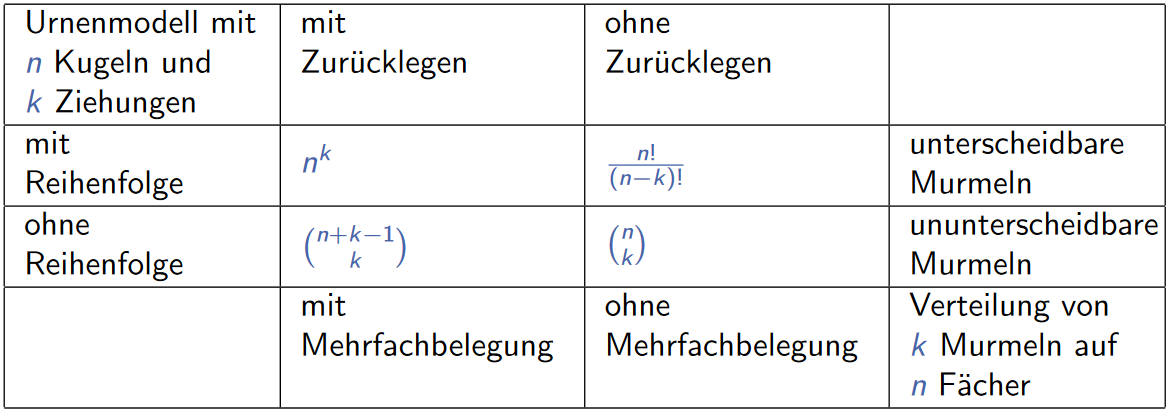
\includegraphics[width=\textwidth]{images/image1.png}
Urnenmodelle ermöglichen es, die Wahrscheinlichkeiten zu bestimmen, falls von einer Gleichverteilung ausgegangen
werden kann!

\paragraph{Definition: Zähldichte}
Sei $(\Omega,\PP)$ ein diskreter Wahrscheinlichkeitsraum.
Dann wird die Funktion
\begin{tightcenter}
	$f:\Omega\rightarrow[0,1], f(\omega)=\PP(\{\omega\})$
\end{tightcenter}
\textbf{Wahrscheinlichkeitsfunktion} oder \textbf{Zähldichte} von $\PP$ genannt.
\newpage
Diese besitzt folgende Eigenschaften:
\begin{itemize}
	\item $\Omega_T\coloneqq\{\omega\in\Omega\mid f(\omega)>0\}$ ist abzählbar und heißt \textbf{Träger} von $\PP$ bzw. von $f$
	\item $\sum\limits_{\omega\in\Omega}f(\omega)=1$
\end{itemize}
Die Zähldichte ist eindeutig!

\paragraph{Definition: Binomialverteilung}
Das Wahrscheinlichkeitsmaß $\PP=Bin_{(n,p)}$ auf $\{0,\ldots,n\}$ mit der Zähldichte
\begin{tightcenter}
	$f(k)=\binom{n}{k}p^k\cdot(1-p)^{n-k}$ \qquad$\forall k\in\{0,\ldots,n\}$
\end{tightcenter}
heißt \textbf{Binomialverteilung} mit Parametern $n\in\N$ und $p\in[0,1]$.

\paragraph{Definition: Geometrische Verteilung}
Das Wahrscheinlichkeitsmaß $\PP=Geo_p$ auf $\N_0$ mit der Zähldichte
\begin{tightcenter}
	$f(k)=(1-p)^k\cdot p$ \qquad$\forall k\in\N_0$
\end{tightcenter}
heißt \textbf{geometrische Verteilung} mit Parameter $p\in(0,1]$.